\section{System Architecture}
In this section, we describe the architecture of the overall system responsible for estimating the position of a user. We will present two approaches; a server-based and a mobile service-based, and describe their respective advantages and disadvantages. Finally, we will compare them in order to make decision on which to approach to implement.

\subsection{Server-Based Architecture}
In a server-based architecture, the position estimation happens on a centralized server, as opposed to locally on the device itself. This architecture introduced some advantages, but also disadvantages.

Since the position estimation happens at a central point, it means that several clients can connect simultaneously to the server. This introduces scalability problems, since one server becomes slower the more clients request a computation from the server. Several techniques can be used to decentralize the computations done by the server in order to make the server scalable. Another problem to consider is server failure. A centralized server is a single point of failure that will affect every client. In order to prevent downtime from server failures, replication is a common technique, where the server is replicated to achieve higher availability. Other examples of failures are transmission failures of messages from or to clients.
This performance and availability, along security and reliability, make up the Quality of Service (QoS).\cite{DS}

The advantage of a server-based architecture is that it makes the application more flexible in terms of updates, such as new \gls{lfp} models. Whenever an update is required to the computation, the update only needs to be applied to the server to affect every client.

\subsection{Mobile Service-Based Architecture}
In a mobile service-based architecture, the whole service would be stored locally on the device. This can be a disadvantage in regards to memory usage. For instance, all the \gls{lfp} models would be stored directly on the device, instead of having them stored on a server. Another disadvantage is when an update is required. For instance, when a new location is added to the application that can be used for indoor positioning, a client must update their application to make use of this new functionality.

Some of the aforementioned disadvantages in a server-based architecture are advantages in a service-based architecture. Since there is no distributed computation to be dependent on, this architecture does not suffer from failures, availability and scalability.
Another advantage is that the development of the application becomes more simple, which induces that the application is easier to implement and maintain.

\subsection{Final Architecture} \label{sec:final_architecture}
Since many of the problems mentioned for a server-based architecture can be resolved with technologies, such as Docker Swarm, and since the application might become heavy in terms of memory usage in a mobile service-based architecture, we will implement our indoor positioning application making use of the server-based architecture.
% Side note: Også fordi vi så er sikre på at opfylde studieordningen.

Using Docker Swarm, we achieve solutions for the problems mentioned with server-based architectures, since its features include scaling, state reconciliation and load balancing\cite{dockerswarm}. Docker Swarm runs Docker containers used to containerize applications. This ensures applications run in the same environment.\cite{docker} The general architecture is seen in \textbf{\autoref{fig:server_architecture}}.

\begin{figure}[H]
    \centering
    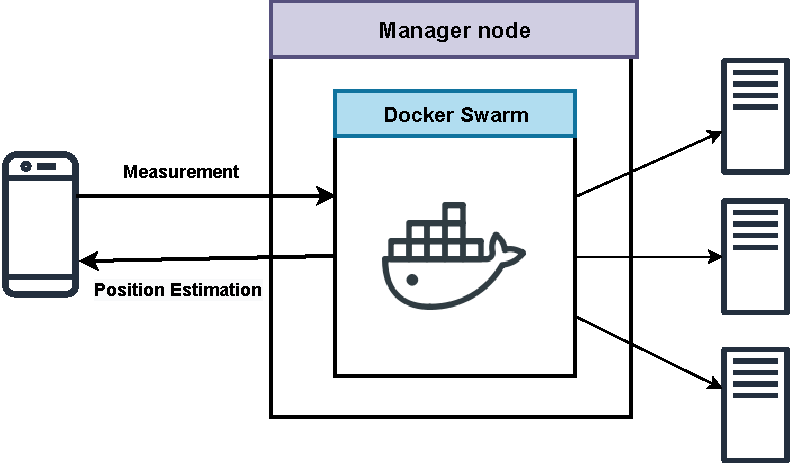
\includegraphics[scale=0.8]{Images/Technology/serverachitectur.pdf}
    \caption{Server-based architecture for indoor positioning system utilizing Docker Swarm.}
    \label{fig:server_architecture}
\end{figure}

To make the server stateless, we must transmit all the necessary history data to the server for each estimation, which is required by the position estimation method. This will of course result in large data transmission the longer the time is spent using the system. Therefore, to optimize data transmission sizes, the client only transmits data from a few steps back. That is, the client transmits all data from last checkpointed position.

In this project, we will focus on the position estimation part of the application. We will implement a server, but not focus on implementing the client-side, as we will prioritise our positioning method instead. Since we argue for a server-based architecture, the bottle neck for our project would be the aforementioned positioning method, and it therefore makes sense to solely focus on the positioning method.